% !TeX program = xelatex
\documentclass[a4paper,10pt]{article}

% ============================================================================
% កញ្ចប់បណ្ណាល័យ (Packages) – តាមលំនាំ NGS Preah Krasang Scenario
% ============================================================================
\usepackage[a4paper, left=0.95cm, right=0.95cm, top=0.80cm, bottom=0.90cm, footskip=0.45cm]{geometry}
\usepackage{amsmath}
\usepackage{unicode-math}
\usepackage{fontspec}
\usepackage{array, longtable, multirow, colortbl}
\usepackage[table]{xcolor}
\usepackage{enumitem}
\usepackage{pifont}
\usepackage{fancyhdr}
\usepackage{tikz}
\usetikzlibrary{calc, arrows.meta, decorations.markings, patterns, babel}

% LaTeX 2025 + longtable v4.24 compatibility guard
\makeatletter
\let\@expl@@@mark@update@singlecol@structures@@\relax
\makeatother

% ============================================================================
% ការកំណត់ពុម្ពអក្សរ (Fonts Configuration - Cross-Platform Windows + Cloud fonts/)
% ============================================================================
\providecommand{\NGSFindFonts}{%
  \IfFileExists{C:/Windows/Fonts/cambria.ttc}{%
    \def\NGSSysPath{C:/Windows/Fonts/}%
    \def\NGSUserPath{C:/Users/KIT/AppData/Local/Microsoft/Windows/Fonts/}%
  }{%
    \IfFileExists{./fonts/KhmerOSsiemreap.ttf}{\def\NGSSysPath{./fonts/}\def\NGSUserPath{./fonts/}}{%
    \IfFileExists{../fonts/KhmerOSsiemreap.ttf}{\def\NGSSysPath{../fonts/}\def\NGSUserPath{../fonts/}}{%
    \IfFileExists{../../fonts/KhmerOSsiemreap.ttf}{\def\NGSSysPath{../../fonts/}\def\NGSUserPath{../../fonts/}}{%
    \IfFileExists{../../../fonts/KhmerOSsiemreap.ttf}{\def\NGSSysPath{../../../fonts/}\def\NGSUserPath{../../../fonts/}}{%
    \IfFileExists{../../../../fonts/KhmerOSsiemreap.ttf}{\def\NGSSysPath{../../../../fonts/}\def\NGSUserPath{../../../../fonts/}}{%
    \IfFileExists{../../../../../fonts/KhmerOSsiemreap.ttf}{\def\NGSSysPath{../../../../../fonts/}\def\NGSUserPath{../../../../../fonts/}}{%
    \IfFileExists{../../../../../../fonts/KhmerOSsiemreap.ttf}{\def\NGSSysPath{../../../../../../fonts/}\def\NGSUserPath{../../../../../../fonts/}}{%
      \def\NGSSysPath{../../../../../../../fonts/}\def\NGSUserPath{../../../../../../../fonts/}%
    }}}}}}}%
  }%
}
\NGSFindFonts

\setmathfont[
  Path={\NGSSysPath},
  FontIndex=1,
  Scale=1.02
]{cambria.ttc}

\defaultfontfeatures{Ligatures=TeX}

\setmainfont[
  Path={\NGSUserPath},
  Extension=.ttf,
  Script=Khmer,
  BoldFont={KhmerOSsiemreap},
  BoldFeatures={FakeBold=1.8},
  ItalicFont={KhmerOSsiemreap},
  ItalicFeatures={FakeSlant=0.25},
  BoldItalicFont={KhmerOSsiemreap},
  BoldItalicFeatures={FakeBold=1.8, FakeSlant=0.25}
]{KhmerOSsiemreap}

\newfontfamily\muol[
  Path={\NGSUserPath},
  Extension=.ttf,
  Script=Khmer
]{KhmerOSmuollight}

\newfontfamily\TimesEn[
  Path={\NGSSysPath},
  Extension=.ttf,
  Scale=1.00,
  BoldFont={timesbd},
  ItalicFont={timesi},
  BoldItalicFont={timesbi}
]{times}

\newfontfamily\NagaBold[
  Path={\NGSUserPath},
  Extension=.ttf
]{AKbalthom Naga Bold}

\newfontfamily\CalibriFont[
  Path={\NGSSysPath},
  Extension=.ttf
]{calibri}

\newfontfamily\CourierBullet[
  Path={\NGSSysPath},
  Extension=.ttf
]{cour}
\newcommand{\wcirc}{{\CourierBullet\fontsize{9.5pt}{11pt}\selectfont o}}

\XeTeXlinebreaklocale "km"
\XeTeXlinebreakskip = 0pt plus 1pt minus 0.1pt

% ============================================================================
% ការកំណត់ពណ៌ និងទម្រង់ទំព័រ (Colors & Page Style)
% ============================================================================
\definecolor{stepgray}{HTML}{D9D9D9}
\definecolor{headgray}{HTML}{F2F2F2}
\definecolor{boxgray}{HTML}{D9D9D9}
\definecolor{darkred}{HTML}{C00000}
\definecolor{red5e}{HTML}{FF0000}

\pagestyle{fancy}
\fancyhf{}
\renewcommand{\headrulewidth}{0pt}
\fancyfoot[R]{\CalibriFont\fontsize{10.5pt}{12pt}\selectfont\thepage}

\setlength{\parindent}{0pt}
\setlength{\parskip}{0pt}
\setlength{\tabcolsep}{3.5pt}
\renewcommand{\arraystretch}{1.14}

\newcolumntype{L}[1]{>{\raggedright\arraybackslash}p{#1}}

% ============================================================================
% ម៉ាក្រូជំនួយ (Helper Macros)
% ============================================================================
\newcommand{\en}[1]{{\TimesEn #1}}
\newcommand{\enbf}[1]{{\TimesEn\textbf{#1}}}
\newcommand{\unit}[1]{\,\text{\en{#1}}}
\newcommand{\fiveE}[1]{{\NagaBold\fontsize{9.5pt}{13pt}\selectfont\textcolor{red5e}{#1}}}
\newcommand{\timenote}[1]{\textcolor{darkred}{\textit{#1}}}
\newcommand{\cnum}[1]{{\fontsize{10pt}{11.5pt}\selectfont\ding{\numexpr181+#1\relax}}}
\newcommand{\ditem}{\tikz[baseline=-0.5ex]\fill (0,0.38ex) -- (0.38ex,0) -- (0,-0.38ex) -- (-0.38ex,0) -- cycle;\hspace{0.25em}}

% រូបផ្ទៀងផ្ទាត់រហ័ស B&W (ក្រឡា (3b)^2=9b^2, ការ៉េបង្វិល 25° (2+3)^2!=13, និងវិសាលភាព -2(a^{-3}b^5)^2)
\newcommand{\figScenarioRefEXP}{%
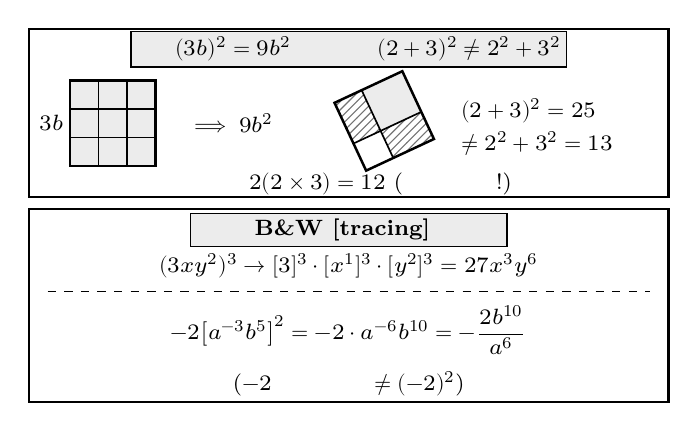
\begin{tikzpicture}[scale=0.95, every node/.style={font=\footnotesize, text=black}]
  % ផ្នែកលើ៖ ក្រឡា 3b x 3b = 9b^2 និងការ៉េបង្វិល 25° (2+3)^2 != 4+9
  \begin{scope}[shift={(0,2.74)}]
    \draw[black, line width=0.9pt] (0,0) rectangle (8.55,2.25);
    \node[fill=gray!15, draw=black, line width=0.5pt, inner sep=2pt] at (4.275,1.98) {\textbf{ក្រឡា} $(3b)^2 = 9b^2$ \textbf{និង អន្ទាក់} $(2+3)^2 \neq 2^2+3^2$};
    % ក្រឡា 3b
    \begin{scope}[shift={(0.55,0.42)}]
      \fill[gray!15] (0,0) rectangle (1.14,1.14);
      \draw[black, line width=0.9pt] (0,0) rectangle (1.14,1.14);
      \draw[black, line width=0.6pt] (0.38,0) -- (0.38,1.14) (0.76,0) -- (0.76,1.14);
      \draw[black, line width=0.6pt] (0,0.38) -- (1.14,0.38) (0,0.76) -- (1.14,0.76);
      \node at (-0.25,0.57) {$3b$};
      \node at (2.15,0.57) {$\implies 9b^2$};
    \end{scope}
    % ការ៉េបង្វិល 25°
    \begin{scope}[shift={(4.75,1.02)}, rotate=25]
      \fill[white] (-0.50,-0.50) rectangle (-0.10,-0.10);
      \fill[gray!15] (-0.10,-0.10) rectangle (0.50,0.50);
      \fill[pattern=north east lines, pattern color=black!55] (-0.50,-0.10) rectangle (-0.10,0.50);
      \fill[pattern=north east lines, pattern color=black!55] (-0.10,-0.50) rectangle (0.50,-0.10);
      \draw[black, line width=0.9pt] (-0.50,-0.50) rectangle (0.50,0.50);
      \draw[black, line width=0.6pt] (-0.10,-0.50) -- (-0.10,0.50) (-0.50,-0.10) -- (0.50,-0.10);
    \end{scope}
    \node[anchor=west] at (5.65,1.15) {$(2+3)^2 = 25$};
    \node[anchor=west] at (5.65,0.72) {$\neq 2^2+3^2 = 13$};
    \node at (4.275,0.18) {បាត់ឆ្នូត $2(2\times 3)=12$ (ហាមបំបែកលើផលបូក!)};
  \end{scope}

  % ផ្នែកក្រោម៖ វិសាលភាពវង់ក្រចក B&W [tracing]
  \begin{scope}[shift={(0,0)}]
    \draw[black, line width=0.9pt] (0,0) rectangle (8.55,2.58);
    \node[fill=gray!15, draw=black, line width=0.5pt, inner sep=2pt] at (4.275,2.30) {\textbf{វិសាលភាព \en{B\&W} [tracing] និងសញ្ញាដក}};
    \node at (4.275,1.82) {$(3xy^2)^3 \to [3]^3\cdot [x^1]^3\cdot [y^2]^3 = 27x^3y^6$};
    \draw[black, line width=0.7pt, dashed] (0.25,1.48) -- (8.30,1.48);
    \node at (4.275,0.96) {$-2\big[a^{-3}b^5\big]^2 = -2\cdot a^{-6}b^{10} = -\dfrac{2b^{10}}{a^6}$};
    \node at (4.275,0.24) {($-2$ នៅក្រៅវង់ក្រចក $\neq (-2)^2$)};
  \end{scope}
\end{tikzpicture}}

\begin{document}
\fontsize{9.8pt}{14.6pt}\selectfont

% ============================================================================
% ក្បាលទំព័រ (Header & Metadata)
% ============================================================================
\begin{center}
{\muol\fontsize{10.4pt}{14pt}\selectfont សេណារីយ៉ូនៃការបង្រៀន \enbf{(}២\enbf{.}៤\enbf{.}១ និង ២\enbf{.}៤\enbf{.}២ ស្វ័យគុណ\enbf{)}}
\end{center}
\vspace{2pt}

\noindent{\setlength{\tabcolsep}{4pt}%
\begin{tabular}{|L{1.75cm}|L{6.65cm}|L{1.85cm}|L{7.55cm}|}
\hline
\rowcolor{headgray}
\textbf{សាលារៀន៖} & អនុវិទ្យាល័យព្រះក្រសាំង (កំពង់ស្វាយ--កំពង់ធំ) & \textbf{មុខវិជ្ជា៖} & គណិតវិទ្យា ថ្នាក់ទី៨ (ពីជគណិត) \\
\hline
\textbf{មេរៀន៖} & \textbf{២.៤.១ ស្វ័យគុណនៃស្វ័យគុណ និង ២.៤.២ ស្វ័យគុណនៃផលគុណ} & \textbf{រយៈពេល៖} & \textcolor{darkred}{\textbf{១ ម៉ោងសិក្សា (៥០ នាទី)}} \textbullet\ ទំ.១៧–១៨ ដើម, ២៥–២៦ \\
\hline
\textbf{គ្រូបង្រៀន៖} & ហុក ប៊ុនថែន & \textbf{កាលបរិច្ឆេទ៖} & \makebox[26mm]{\dotfill}\ ២០២៦ (ព.ស. ២៥៧០) \\
\hline
\end{tabular}}

\vspace{3pt}
{\muol ផ្នែកទី ១៖ លំដាប់ឈុតឆាកបង្រៀន ៥០ នាទី \enbf{(}៨ ឈុតលម្អិត\enbf{)}}
\vspace{1pt}

% ============================================================================
% ផ្នែកទី ១៖ តារាងឈុតឆាក (8 Chronological Scenes = 50 min)
% ============================================================================
\begin{longtable}{|c|L{2.75cm}|c|L{7.65cm}|L{4.45cm}|}
\hline
\rowcolor{stepgray}
\textbf{ម៉ោង} & \textbf{ឈុត / ជំហាន \enbf{5E}} & \textbf{នាទី} & \textbf{សកម្មភាពបង្រៀន និងសំណួរ--ចម្លើយគំរូ (គ្រូ--សិស្ស)} & \textbf{សម្ភារៈ និងកំណត់ចំណាំ / \enbf{Warrant}} \\
\hline
\endfirsthead
\hline
\rowcolor{stepgray}
\textbf{ម៉ោង} & \textbf{ឈុត / ជំហាន \enbf{5E}} & \textbf{នាទី} & \textbf{សកម្មភាពបង្រៀន និងសំណួរ--ចម្លើយគំរូ (គ្រូ--សិស្ស)} & \textbf{សម្ភារៈ និងកំណត់ចំណាំ / \enbf{Warrant}} \\
\hline
\endhead
\hline
\endfoot
\hline
\endlastfoot

00--02 &
\textbf{ឈុតទី ១}\par
ជំហានទី១៖ រដ្ឋបាលថ្នាក់ &
២ &
\ditem គ្រូពិនិត្យអវត្តមាន និងបែងចែកសិស្សជា \textbf{«ក្រុមវិស្វករអង្គចងចាំ និងការ៉ូ ៣ តួនាទី»} (៣ នាក់/ក្រុម) ។\par
\ditem \textbf{គ្រូ៖} «ដាក់កន្ត្រៃ និងបន្ទាត់រាបស្មើលើតុ ហើយផ្កាប់សន្លឹក ១:១ មុនពេលចាប់ផ្ដើម!» \par
\textbf{សិស្ស៖} អនុវត្តតាម។ &
\wcirc\ កំណត់វិន័យកន្ត្រៃ/បន្ទាត់។\par
\wcirc\ ចែកសន្លឹក \en{P1 1:1} ផ្កាប់មុខ។ \\
\hline

02--08 &
\textbf{ឈុតទី ២}\par
ជំហានទី២៖ កំណែ និងរំលឹកមេរៀនចាស់ &
៦ &
\ditem \textbf{ក. កំណែ ($\le 3\unit{min}$, ប្រតិបត្តិ ទំ.១៦)៖} ផ្ទៀង ក. $\frac{x^9}{x^4}=x^5$ ($x\neq 0$), ខ. $\frac{(3/2)^2}{(3/2)^4}=\left(\frac{3}{2}\right)^{-2}$, គ. $\frac{y^9}{y^9}=y^0=1$ ($y\neq 0$), ឃ. $\left(\frac{3yx^9}{-15y^5x^4}\right)^0=1$ ($x,y\neq 0$) ។\par
\textbf{គ្រូ៖} «ក្នុង ឃ ហេតុអ្វីមិនបាច់សម្រួលក្នុងវង់ក្រចក?» \par
\textbf{សិស្ស៖} «ព្រោះស្វ័យគុណ $0$ នៃកន្សោមខុសពីសូន្យស្មើ $1$ ភ្លាម!» &
\wcirc\ រក្សាកំណែ $\le 3$ នាទី។\par
\wcirc\ ផ្ដោតអន្ទាក់ស្វ័យគុណ $0$ (\cnum{5})។ \\[3pt]

& & &
\ditem \textbf{ខ. រំលឹក (៣នាទី, ទំ.១៥)៖} $a^n = a\cdot a\cdots a$ ($n$ កត្តា), $a^{-n} = \frac{1}{a^n}$ ($a\neq 0$), និង $a^m\cdot a^n = a^{m+n}$ (ឧ. $2^3\cdot 2^4 = 2^7$) ។ &
\wcirc\ \en{Warrant} \cnum{4}, \cnum{5}៖ រំលឹកច្បាប់គោលដូចគ្នាមុនភ្ជាប់ $(2^3)^4$។ \\
\hline

08--11 &
\textbf{ឈុតទី ៣}\par
\fiveE{E1 Engage}\par
បន្ទះអង្គចងចាំ និងការ៉ូការេ &
៣ &
\ditem \textbf{ស្ថានភាពទី១ (៤.១)៖} កញ្ចប់ទិន្នន័យ $(2^3)^4$ បៃ — សុខថា $(2^3)^4 = 2^{3+4} = 2^7 = 128$; បូណាថា $(2^3)^4 = 2^{3\times 4} = 2^{12} = 4\,096$ ។ \par
\ditem \textbf{ស្ថានភាពទី២ (៤.២)៖} ការេធំជ្រុង $(3b)\unit{cm}$ ផ្សំពីការ៉ូជ្រុង $b\unit{cm}$ — សុខថា $(3b)^2 = 3b^2$ ($3$ ការ៉ូ); បូណាថា $(3b)^2 = 9b^2$ ($9$ ការ៉ូ) ។ &
\wcirc\ សួរទស្សន៍ទាយមុន មិនទាន់លាតចម្លើយ។ \\[3pt]

& & &
\textbf{គ្រូ៖} «តើក្រុមប្អូនជឿសុខ ឬបូណាក្នុងស្ថានភាពទាំងពីរ?» \par
\textbf{សិស្ស៖} បោះឆ្នោតទស្សន៍ទាយខុសៗគ្នា ហើយគ្រូកត់សម្គាល់លើក្ដារខៀនទុកផ្ទៀងនៅ \fiveE{E5}។ &
\wcirc\ កត់ត្រាការទស្សន៍ទាយទុកផ្ទៀងនៅ \fiveE{E5}។ \\
\hline

11--22 &
\textbf{ឈុតទី ៤}\par
\fiveE{E2 Explore}\par
\en{Dual POE} ១:១ (\en{5m + 6m}) &
១១ &
\ditem \textbf{ស្ថានីយទី១ (\en{POE 1} ៤.១, ៥នាទី, \en{P1 1:1})៖} ផ្ទៀងក្រិត $5.0\unit{cm}$ កាត់ ៤ បន្ទះកញ្ចប់ $2^3$ ($3\unit{cm}$/បន្ទះ $\to 12\unit{cm}$) អូស \en{[tracing]}៖ ក. $(2^3)^4 = 2^{3+3+3+3} = 2^{3\times 4} = 2^{12}$; ខ. $(5^6)^4 = 5^{24}$ និង $(2^3)^4 = (2^4)^3 = 2^{12}$ ។\par
\textbf{អន្ទាក់ប្រៀបធៀប៖} $2^3\cdot 2^4 = 2^7$ (បូក) $\neq (2^3)^4 = 2^{12}$ (គុណឆ្លងវង់ក្រចក)។ &
\wcirc\ សន្លឹក \en{P1 1:1} (\en{Actual Size 100\%})។\par
\wcirc\ បង្គាប់អូស \en{[tracing]} រាប់ $12$ ប្លុក។ \\[3pt]

& & &
\ditem \textbf{ស្ថានីយទី២ (\en{POE 2} ៤.២, ៦នាទី, \en{P1 1:1})៖}\par
\textbf{ផ្នែក \en{A} (ទំ.១៧ ក, ខ, គ)៖} ក. $2^3\cdot 5^3 = (2\cdot 5)^3 = 10^3 = 1\,000$; ខ. $2^2\cdot 5^2\cdot 7^2 = (2\cdot 5\cdot 7)^2 = 70^2 = 4\,900$; គ. $a^n b^n = (ab)^n$ ។\par
\textbf{ផ្នែក \en{B}៖} ក្រឡា $6\times 6\unit{cm}$ ($b=2\unit{cm}$, ជ្រុង $3b$) $\to 9b^2 \neq 3b^2$ និងការ៉េបង្វិល $25^\circ$៖ $(2+3)^2 = 25 \neq 2^2+3^2 = 13$ (បាត់ $2\times 6 = 12$)! &
\wcirc\ បង្កើតជម្លោះយល់ដឹង៖ រូបភាពបង្ហាញ $9$ ការ៉ូ និងផ្នែកបាត់ $12$។ \\
\hline

22--28 &
\textbf{ឈុតទី ៥}\par
\fiveE{E3 Explain}\par
ទ្រឹស្ដីបទ «ជាទូទៅ» និង \cnum{1}--\cnum{5} &
៦ &
\ditem សិស្សបង្គុំប្រអប់ \textbf{«ជាទូទៅ» ៤.១ និង ៤.២ (ទំ.១៧)} រួមទាំងលក្ខខណ្ឌ $a\neq 0, b\neq 0$ ពេលនិទស្សន្ត $\le 0$ ៖\par
$(a^m)^n = (a^n)^m = a^{m\cdot n}$ \quad និង \quad $(a\cdot b)^n = a^n\cdot b^n$ ។\par
\ditem សង្ខេបតារាង \textbf{សម្មតិកម្ម--សន្និដ្ឋាន--វិបាក} ($a^nb^n=(ab)^n$, $(a+b)^n\neq a^n+b^n$) និងសួរសំណួរ \en{Beeth} ៣ ជំហាន (យល់-ទូលាយ-សមហេតុផល)។ &
\wcirc\ ផ្ទាំង \textbf{\en{Warrant Bank} \cnum{1}--\cnum{5} (\en{P4})}៖\par
\cnum{1} $(a^m)^n=(a^n)^m=a^{mn}$\par
\cnum{2} $(ab)^n=a^n b^n$ (ចែក) \\[3pt]

& & &
\ditem បិទផ្ទាំង \textbf{ធនាគារហេតុផល \cnum{1}--\cnum{5} (\en{P4})}៖ \cnum{1} ស្វ័យគុណនៃស្វ័យគុណ, \cnum{2} ចែកនិទស្សន្ត, \cnum{3} ផ្គុំគោលគុណ, \cnum{4} ផលគុណគោលដូចគ្នា ($a=a^1$), \cnum{5} និទស្សន្តដក/សូន្យ និង $-c(ab)^n \neq (-cab)^n$ ។ &
\cnum{3} $a^nb^n=(ab)^n$ (ផ្គុំ)\par
\cnum{4} $a^ma^n=a^{m+n}, a=a^1$\par
\cnum{5} $a^{-n}, a^0, -c(ab)^n$។ \\
\hline

28--38 &
\textbf{ឈុតទី ៦}\par
\fiveE{E4 Elaborate}\par
កាតស៊ើបអង្កេត ៣ ជំហាន &
១០ &
\ditem ចែកកាត \textbf{\en{P2}} ព័ទ្ធវង់ក្រចក \en{[tracing]} $\to$ \cnum{1}--\cnum{5} $\to$ គណនា៖\par
\textbf{គំរូ ៤.១ (ទំ.១៧)៖} ក. $(10^2)^3 = 10^6 = 1\,000\,000$ (\cnum{1}); ខ. $(a^{-2})^k(a^k)^5 = a^{-2k}\cdot a^{5k} = a^{3k}$ (\cnum{1}, \cnum{4}; $a\neq 0$) ។\par
\textbf{គំរូ ៤.២ (ទំ.១៨ ដើម)៖} ក. $(3xy^2)^3 \to [3]\cdot[x^1]\cdot[y^2] \implies 27x^3y^6$ (\cnum{2}, \cnum{1}); ខ. $(b^3)(b^{2k-1})^3 = b^3\cdot b^{6k-3} = b^{6k}$ (\cnum{1}, \cnum{4}; $b\neq 0$) ។ &
\wcirc\ \en{P2} បង្ហាញស៊ុមប្រៀបធៀប $(-2a^{-3}b^5)^2$ vs $-2(a^{-3}b^5)^2$។ \\[3pt]

& & &
\ditem \textbf{\en{EIA Looking-Back}៖}\par
១) ហេតុអ្វី $(3xy^2)^3 = 3x^3y^6$ ឬ $9x^3y^5$ ខុស?\par
២) ហេតុអ្វី $b^{3(2k-1)} \neq b^{6k-1}$?\par
\textbf{សិស្ស៖} «ភ្លេចលើក $3^3=27$ និងត្រូវគុណ $3$ លើតួ $-1$ ផង!» &
\wcirc\ ប្រើ \en{Warrant} \cnum{1}, \cnum{2}, \cnum{4} និង \en{[tracing]} តាមកត្តា។ \\
\hline

38--48 &
\textbf{ឈុតទី ៧}\par
\fiveE{E5 Evaluate}\par
\en{Relay}, បិទ \en{E1}, កាត \en{A--D} &
១០ &
\ditem \textbf{\en{Relay} ៣ តួនាទី (៦នាទី, \en{P3}) — បេសកកម្ម \en{A} (៤.១ ទំ.១៧)៖}\par
ក. $(a^3)^{-2}=a^{-6}=\frac{1}{a^6}$ (\cnum{1}, \cnum{5}); ខ. $a(a^4)^5 a^{-6}=a^{15}$ (\cnum{1}, \cnum{4}; $a\neq 0$) ។\par
\textbf{គ្រូ៖} «តួនាទី ១ អូស \en{[tracing]} ហើយហៅ \en{Pause-Ask!} មុនឱ្យតួនាទី ២ គណនា!» &
\wcirc\ តួនាទី ១៖ \en{[tracing]} + \en{Pause-Ask!}\par
\wcirc\ តួនាទី ២៖ \cnum{1}--\cnum{5} និងគណនា \\[3pt]

& & &
\ditem \textbf{បេសកកម្ម \en{B} (៤.២ ទំ.១៨ ដើម)៖}\par
ក. $-2(a^{-3}b^5)^2 = -2a^{-6}b^{10} = -\frac{2b^{10}}{a^6}$ (\cnum{5}, \cnum{2}, \cnum{1}; $a\neq 0$);\par
ខ. $a(a^4)a^{-6} = a^{-1} = \frac{1}{a}$ (\cnum{4}, \cnum{5}; បញ្ជាក់ពុម្ពទំ.១៨ បាត់និទស្សន្ត $5$) ។\par
\textbf{សិស្ស៖} «$-2$ នៅក្រៅវង់ក្រចក មិនលើកស្វ័យគុណ $2$ ទេ!» &
\wcirc\ តួនាទី ៣៖ ផ្ទៀងសញ្ញាដក និងលក្ខខណ្ឌ $a\neq 0$ (\en{Pause-Review!})។ \\[3pt]

& & &
\ditem \textbf{បិទ \en{E1} (១.៥នាទី)៖} បូណាត្រូវទាំងពីរ ($(2^3)^4=2^{12}=4\,096$ និង $(3b)^2=9b^2$) ។\par
\ditem \textbf{កាតវិនិច្ឆ័យ \en{A--D} និង \en{Exit Ticket} (២.៥នាទី, \en{P5})៖} \en{A:} $(x^4)^3=x^7$ (\ding{55}), \en{B:} $(-2x^3y)^2=-2x^6y^2$ (\ding{55}), \en{C:} $(-2x^3y)^2=4x^6y^2$ (\ding{51}), \en{D:} $(x+y)^3=x^3+y^3$ (\ding{55}) ។ &
\wcirc\ ត្រួតពិនិត្យចម្លើយ \en{A--D} ភ្លាមៗ និងប្រមូលសំបុត្រចេញ ៩០ វិនាទី។ \\
\hline

48--50 &
\textbf{ឈុតទី ៨}\par
ជំហានទី៥៖ កិច្ចការផ្ទះ &
២ &
\ditem ប្រគល់ប័ណ្ណកិច្ចការផ្ទះ \textbf{\en{P6} (ទំ.២៥–២៦)}៖\par
• \textbf{ផ្នែក ក៖} ១) គណនា $(4^3)(2^2)$ ដោយប្ដូរ $4=2^2$ ($2^8=256$) និង $25^3\cdot 4^3$ ដោយ \cnum{3} ($100^3=1\,000\,000$); ២) សម្រួល $(-2a^2x^2)^2(-4a^3x)^3 = -256a^{13}x^7$ (ត្រៀម \#7ង) ។\par
• \textbf{ផ្នែក ខ (\#8ក,ខ,គ)៖} $x^{12}=(x^2)^6$, $y^{15}=(y^3)^5$, $2^{18}=8^6$, $(2^5)^6=8^{10}$ ។ &
\wcirc\ ផ្ទៀងលេខលំហាត់លើ \en{P6}។\par
\wcirc\ ប្រកាសមេរៀនបន្ទាប់៖ \textbf{៤.៣ ស្វ័យគុណនៃផលចែក (ទំ.១៨–១៩)}។ \\
\hline
\end{longtable}

\vspace{2pt}
% ============================================================================
% ផ្នែកទី ២ & ផ្នែកទី ៣ (Side-by-Side Minipages — លំនាំ Teaching_Scenario_INEQ1)
% ============================================================================
\noindent\begin{minipage}[t]{0.46\textwidth}
{\muol ផ្នែកទី ២៖ បញ្ជីសម្ភារៈ \enbf{B\&W} និងរូបផ្ទៀងផ្ទាត់រហ័ស}\\[2pt]
{\fontsize{8.5pt}{12.0pt}\selectfont
\ditem \textbf{\en{P1} (១ សន្លឹក/ក្រុម, \en{1:1})៖} ក្រិត $5.0\unit{cm}$, ៤ បន្ទះ $2^3$ ($3\unit{cm}$) + ថាស $12\unit{cm}$, ក្រឡា $6\times 6\unit{cm}$ ($3b\times 3b$), ការ៉េបង្វិល $(2+3)^2$ ។\par
\ditem \textbf{\en{P2} និង \en{P3}៖} កាតស៊ើបអង្កេត \en{E4} (គំរូ ៤.១–៤.២) និងសន្លឹក \en{Relay E5} ៣ តួនាទី (ប្រតិបត្តិ ទំ.១៧–១៨) ។\par
\ditem \textbf{\en{P4, P5, P6}៖} ផ្ទាំង \textbf{\en{Warrant Bank} \cnum{1}--\cnum{5}}, កាត \en{A--D} + \en{Exit Ticket}, ប័ណ្ណកិច្ចការផ្ទះ ទំ.២៥–២៦ ។\par
\ditem \textbf{ឧបករណ៍៖} កន្ត្រៃ បន្ទាត់ ១:១ និងខ្មៅដៃ \en{[tracing]} ។\par
\vspace{2pt}
{\centering\figScenarioRefEXP\par}
\vspace{1pt}
\raggedright\textbf{ចំណាំ \en{Warrant}៖} \cnum{1} $(a^m)^n=a^{mn}$ $\mid$ \cnum{2} $(ab)^n=a^n b^n$ $\mid$ \cnum{3} $a^n b^n=(ab)^n$ $\mid$ \cnum{4} $a^m a^n=a^{m+n}, a=a^1$ $\mid$ \cnum{5} $a^{-n}, a^0, -c(ab)^n$ ។}
\end{minipage}\hfill
\begin{minipage}[t]{0.51\textwidth}
{\muol ផ្នែកទី ៣៖ ការភាន់ច្រឡំសិស្ស និងវិធានការដោះស្រាយ}\\[2pt]
{\fontsize{8.3pt}{11.8pt}\selectfont\renewcommand{\arraystretch}{1.08}%
\begin{tabular}{|L{3.50cm}|L{5.60cm}|}
\hline
\rowcolor{stepgray}
\textbf{ការភាន់ច្រឡំសិស្ស (\en{Empirical})} & \textbf{វិធានការបង្ការ និងដោះស្រាយក្នុងថ្នាក់} \\
\hline
\textbf{១. បូកនិទស្សន្តក្នុង $(a^m)^n$៖} សរសេរ $(2^3)^4=2^7$ ឬ $(x^4)^3=x^7$ (\en{Ulusoy, 2019}: 8.4\%–24.8\%; \en{Şenay, 2024}: 34\%) ។ & ប្រើ \textbf{\en{P1 1:1}} កាត់ ៤ បន្ទះ $2^3$ ដាក់លើថាស $12\unit{cm}$ ផ្ទៀង $2^{12}\neq 2^7$, ប្រៀបធៀបឆ្លងវង់ក្រចក \cnum{1} vs គោលដូចគ្នា \cnum{4} ។ \\
\hline
\textbf{២. បំបែកស្វ័យគុណលើផលបូក៖} គិតថា $(a+b)^n = a^n+b^n$ (\en{Theba et al., 2024}: 60.3\%; \en{Larbi \& Mavis, 2016}) ។ & បង្ហាញក្រឡា \textbf{\en{P1 1:1}} $(3b)^2=9b^2$ និងការ៉េបង្វិល $25^\circ$ $(2+3)^2=25 \neq 4+9=13$ រកផ្នែកបាត់ $12$ + កាតអន្ទាក់ \textbf{\en{D}} ។ \\
\hline
\textbf{៣. ភ្លេចមេគុណក្នុង $(ab)^n$៖} សរសេរ $(3xy^2)^3 = 3x^3y^6$ (\en{Booth et al., 2014}: ~0.80/សិស្ស; \en{Ngo et al., 2023}) ។ & ព័ទ្ធវង់ក្រចក \en{B\&W} $[3]\cdot[x^1]\cdot[y^2]$ (\en{P2}) + \en{[tracing]} (\en{Yeo \& Tzeng, 2019}) + \en{EIA Looking-Back} ។ \\
\hline
\textbf{៤. សញ្ញាដកក្រៅវង់ក្រចក និង $a^0$៖} ច្រឡំ $-2(a^{-3}b^5)^2$ ជា $(-2)^2$ ឬ $-3^0=1$ (\en{Olson et al., 2011}: 6/19; \en{Ulusoy, 2019}: 66.1\%) ។ & ប្រើ \cnum{5} ញែក $-2[a^{-3}b^5]^2$ vs $[-2x^3y]^2$, វិន័យ \en{Pause-Ask / Pause-Review} (\en{P3}), និងកាត \textbf{\en{B vs C}} (\en{P5}) ។ \\
\hline
\end{tabular}}
\end{minipage}

\vspace{8pt}
% ============================================================================
% ផ្នែកទី ៤៖ ប្លង់គ្រប់គ្រងក្ដារខៀន ៣ ភាគ (Board Management Plan)
% ============================================================================
{\muol ផ្នែកទី ៤៖ ប្លង់គ្រប់គ្រងក្ដារខៀន ៣ ភាគ}\\[3pt]
{\fontsize{8.5pt}{12.4pt}\selectfont\renewcommand{\arraystretch}{1.14}%
\begin{tabular}{|L{6.00cm}|L{6.25cm}|L{6.00cm}|}
\hline
\rowcolor{stepgray}
\textbf{ក្ដារខៀនឆ្វេង៖ ទ្រឹស្ដី «ជាទូទៅ» និង \en{Warrant} \cnum{1}--\cnum{5}} &
\textbf{ក្ដារខៀនកណ្ដាល៖ ការសង្កេត \en{E2} និងគំរូ \en{E4}} &
\textbf{ក្ដារខៀនស្ដាំ៖ \en{E1, Relay E5} និងបិទមេរៀន} \\
\hline
\textbf{៤.១ ស្វ័យគុណនៃស្វ័យគុណ (ទំ.១៧)៖}\par
$(a^m)^n = (a^n)^m = a^{mn}$ \quad (\cnum{1})\par
\textbf{៤.២ ស្វ័យគុណនៃផលគុណ (ទំ.១៧)៖}\par
$(a\cdot b)^n = a^n\cdot b^n$ (\cnum{2}) \textbar{} $a^n b^n=(ab)^n$ (\cnum{3})\par
\textit{លក្ខខណ្ឌ៖} $a\neq 0, b\neq 0$ ករណីនិទស្សន្ត $\le 0$\par
\textbf{ហេតុផលបន្ថែម៖}\par
\cnum{4} $a^m a^n=a^{m+n},\; a=a^1$ \par
\cnum{5} $a^{-n}=\frac{1}{a^n},\; a^0=1,\; -c(ab)^n\neq(-cab)^n$
&
\textbf{ពិសោធន៍ \en{POE 1--2} (\en{E2})៖}\par
• $(2^3)^4 = 2^{3\times 4}=2^{12}$ $\neq 2^3\cdot 2^4 = 2^7$\par
• $(3b)^2 = 9b^2$ \textbar{} $(2+3)^2=25\neq 4+9=13$\par
\textbf{លំហាត់គំរូ ៤.១–៤.២ (\en{E4})៖}\par
• $(10^2)^3 = 10^6 = 1\,000\,000$\par
• $(a^{-2})^k(a^k)^5 = a^{-2k+5k}=a^{3k}$ ($a\neq 0$)\par
• $(3xy^2)^3 = [3]^3[x^1]^3[y^2]^3 = 27x^3y^6$\par
• $b^3(b^{2k-1})^3 = b^3 b^{6k-3}=b^{6k}$ ($b\neq 0$)
&
\textbf{បេសកកម្ម \en{E1} (កត់ត្រាទស្សន៍ទាយដើមម៉ោង)៖}\par
• សុខ vs បូណា៖ $(2^3)^4$ និង $(3b)^2$ $\to$ បូណាត្រូវ!\par
\textbf{លទ្ធផល \en{Relay E5} (ទំ.១៧–១៨)៖}\par
• \en{A}: $(a^3)^{-2}=\frac{1}{a^6}$ \textbar{} $a(a^4)^5 a^{-6}=a^{15}$\par
• \en{B}: $-2(a^{-3}b^5)^2=-\frac{2b^{10}}{a^6}$ \textbar{} $a(a^4)a^{-6}=\frac{1}{a}$\par
\textbf{ត្រួតពិនិត្យ \en{A--D} និង \en{P6}៖}\par
ចម្លើយត្រូវ \en{C} \textbar{} កិច្ចការផ្ទះ៖ ទំ.២៥–២៦ \\
\hline
\end{tabular}}

\end{document}
